\Transcb{yellow}{blue}{Neutrinos van kosmische gammaflitsen}
\twocolumn
\begin{itemize}
\item Signalen zijn atm. achtergrond $\nu$
\item[] Niet te onderscheiden van kosm. $\nu$
\item {\blue Langer meten $\rightarrow$ Hot spots}
\item Of : \colorbox{yellow}{Kijk naar kortstondige explosies}
\item[] Specifieke plaats en tijd (satelliet)
\item[] $\rightarrow$ nagenoeg geen achtergrond
\item Gelijktijdig $\gamma - \nu$ signaal
\item[] Faalt ingeval van een tijdverschil
\item \colorbox{yellow}{@VUB: Nieuwe methode}
\item[] Ontwikkeld voor $\gamma - \nu$ tijdverschillen
\item[] Stapelt info van diverse bursts
\end{itemize}

\newpage

\begin{center}
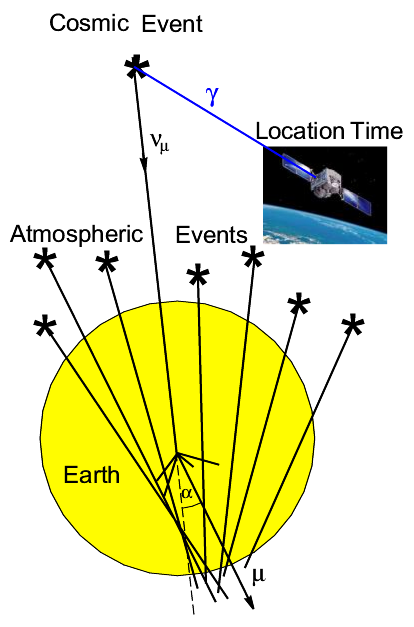
\includegraphics[keepaspectratio,height=16cm]{atm-bkg}
\end{center}
